\documentclass[12pt]{article}
\usepackage[utf8]{inputenc} % For UTF-8 encoding
\usepackage{amsmath, amssymb, amsthm} % For mathematical formatting
\usepackage{multirow} % For multirow in tables
\usepackage[a4paper, margin=0.75in]{geometry} % For setting page size and margins
\usepackage{xcolor, listings} % For code highlighting
\usepackage{longtable} % For long tables
\usepackage{graphicx} % For including images
\setlength{\parindent}{0pt}


\title{Computer Architecture HW 4}
\author{111062117, Hsiang-Sheng Huang}

\begin{document}

\maketitle

\begin{figure}[h!]
    \centering
    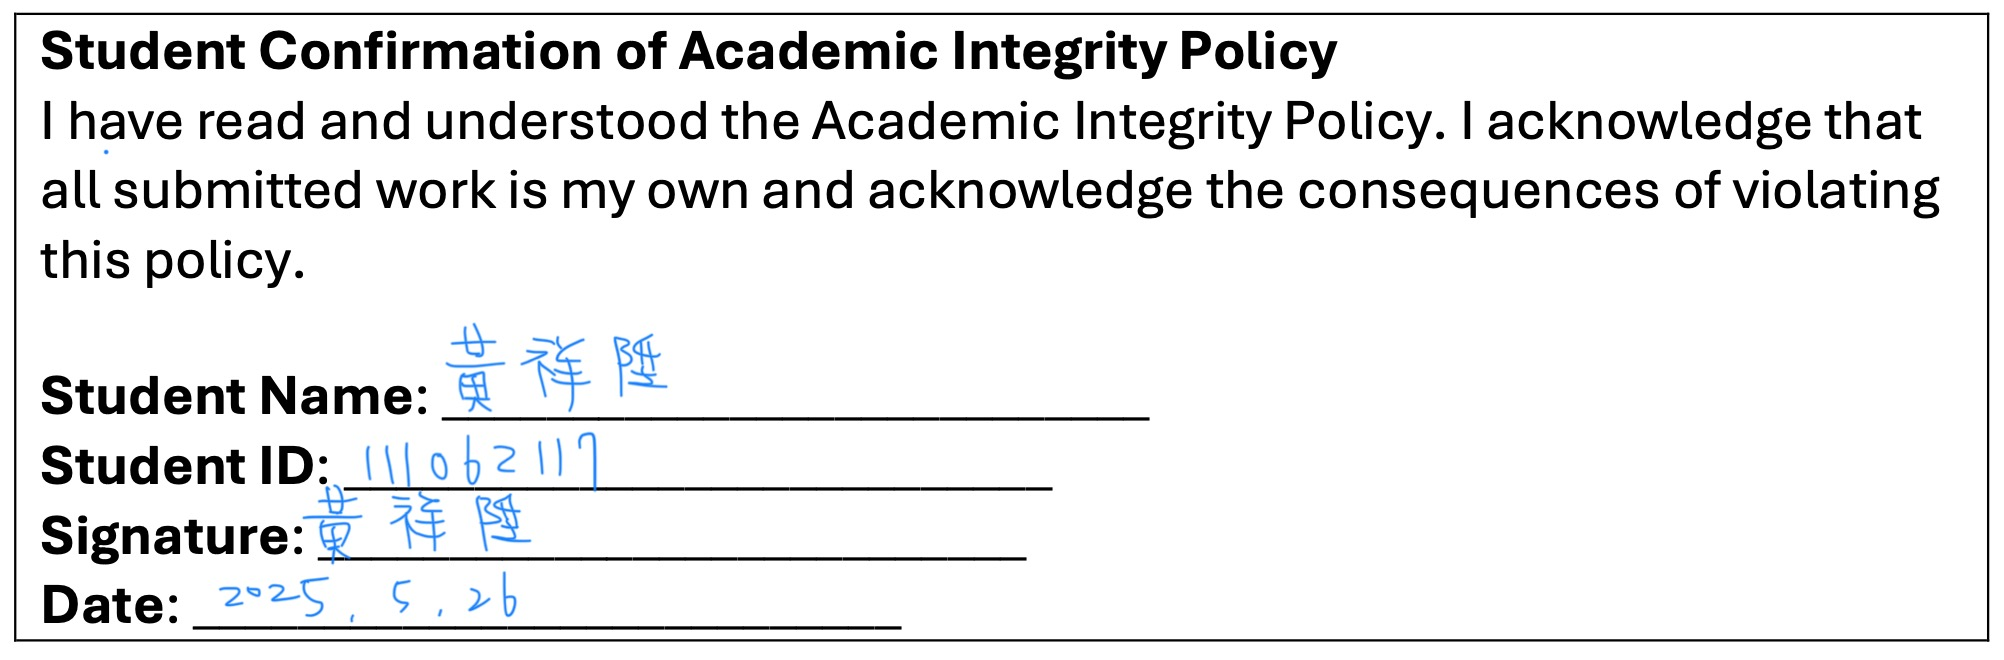
\includegraphics[width=0.8\textwidth]{./img/signature.png}
\end{figure}

\begin{center}
    \large \textbf{Part A: Coding and Simulation}
\end{center}

\section*{1}

\subsection*{(1) RISC-V assembly code}

This section is provided in the attached file \texttt{HW5\_MCM\_111062117.S}.

\subsection*{(2) Flowchart and evidence of correct results}

\begin{figure}[h!]
    \centering
    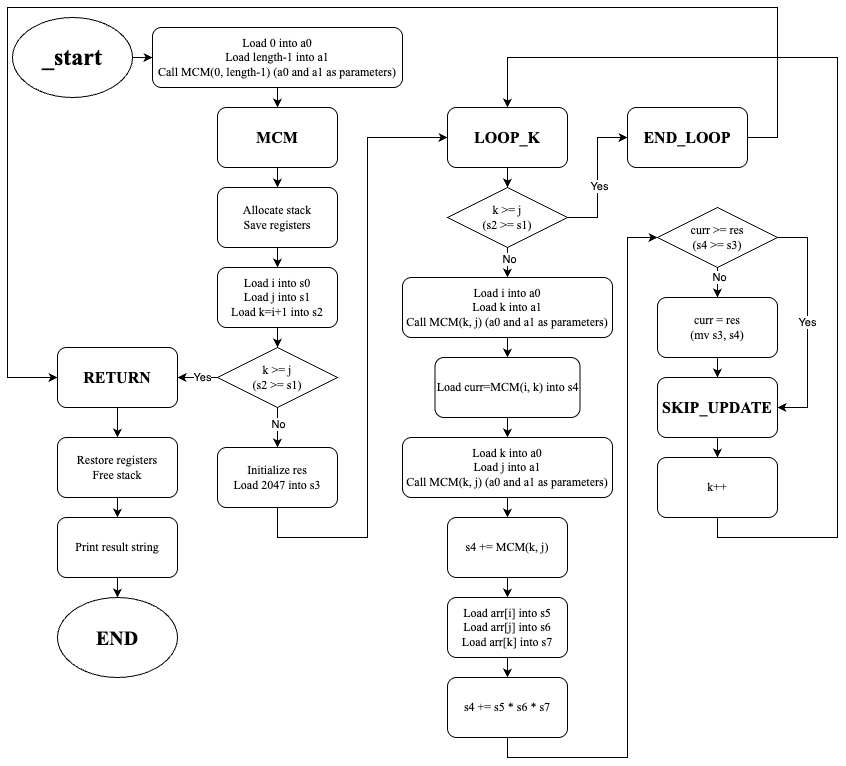
\includegraphics[width=0.8\textwidth]{./img/flowchart.png}
    \caption{Flowchart of the MCM assembly code}
\end{figure}

\begin{figure}[h!]
    \centering
    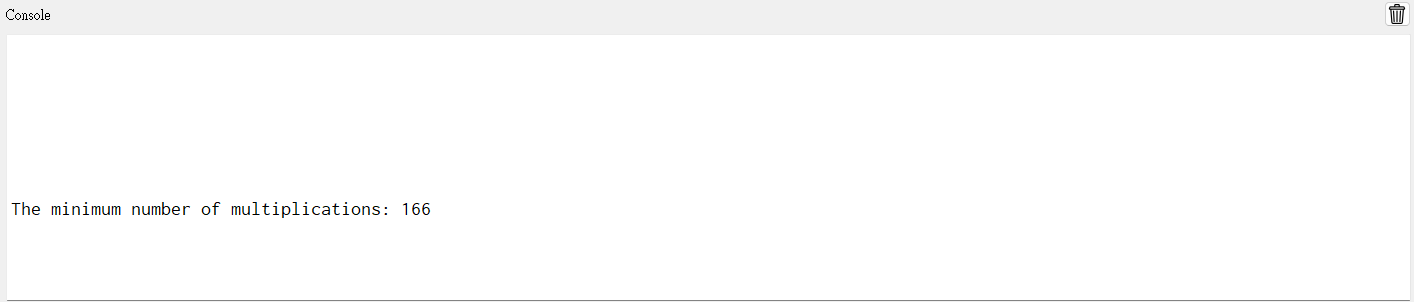
\includegraphics[width=0.8\textwidth]{./img/correct_1.png}
    \caption{Evidence of correct results (testcase 1)}
\end{figure}

\begin{figure}[h!]
    \centering
    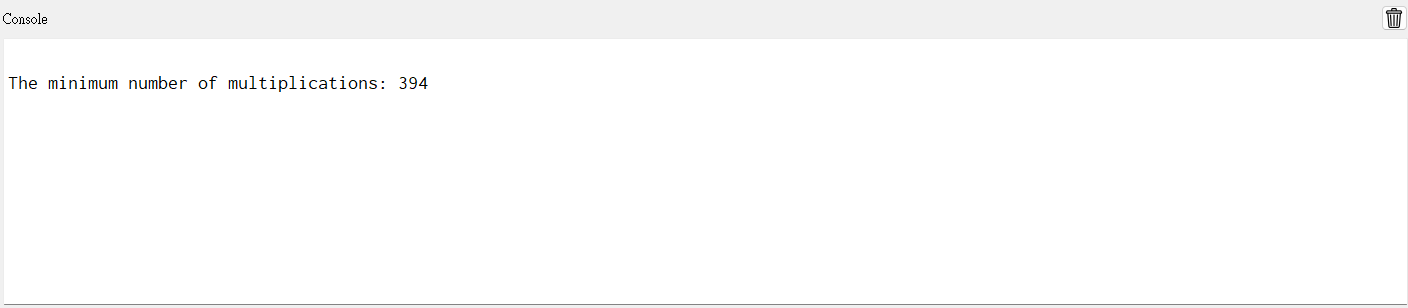
\includegraphics[width=0.8\textwidth]{./img/correct_2.png}
    \caption{Evidence of correct results (testcase 2)}
\end{figure}

\clearpage

\section*{2}

\subsection*{(a)}

\begin{figure}[h!]
    \centering
    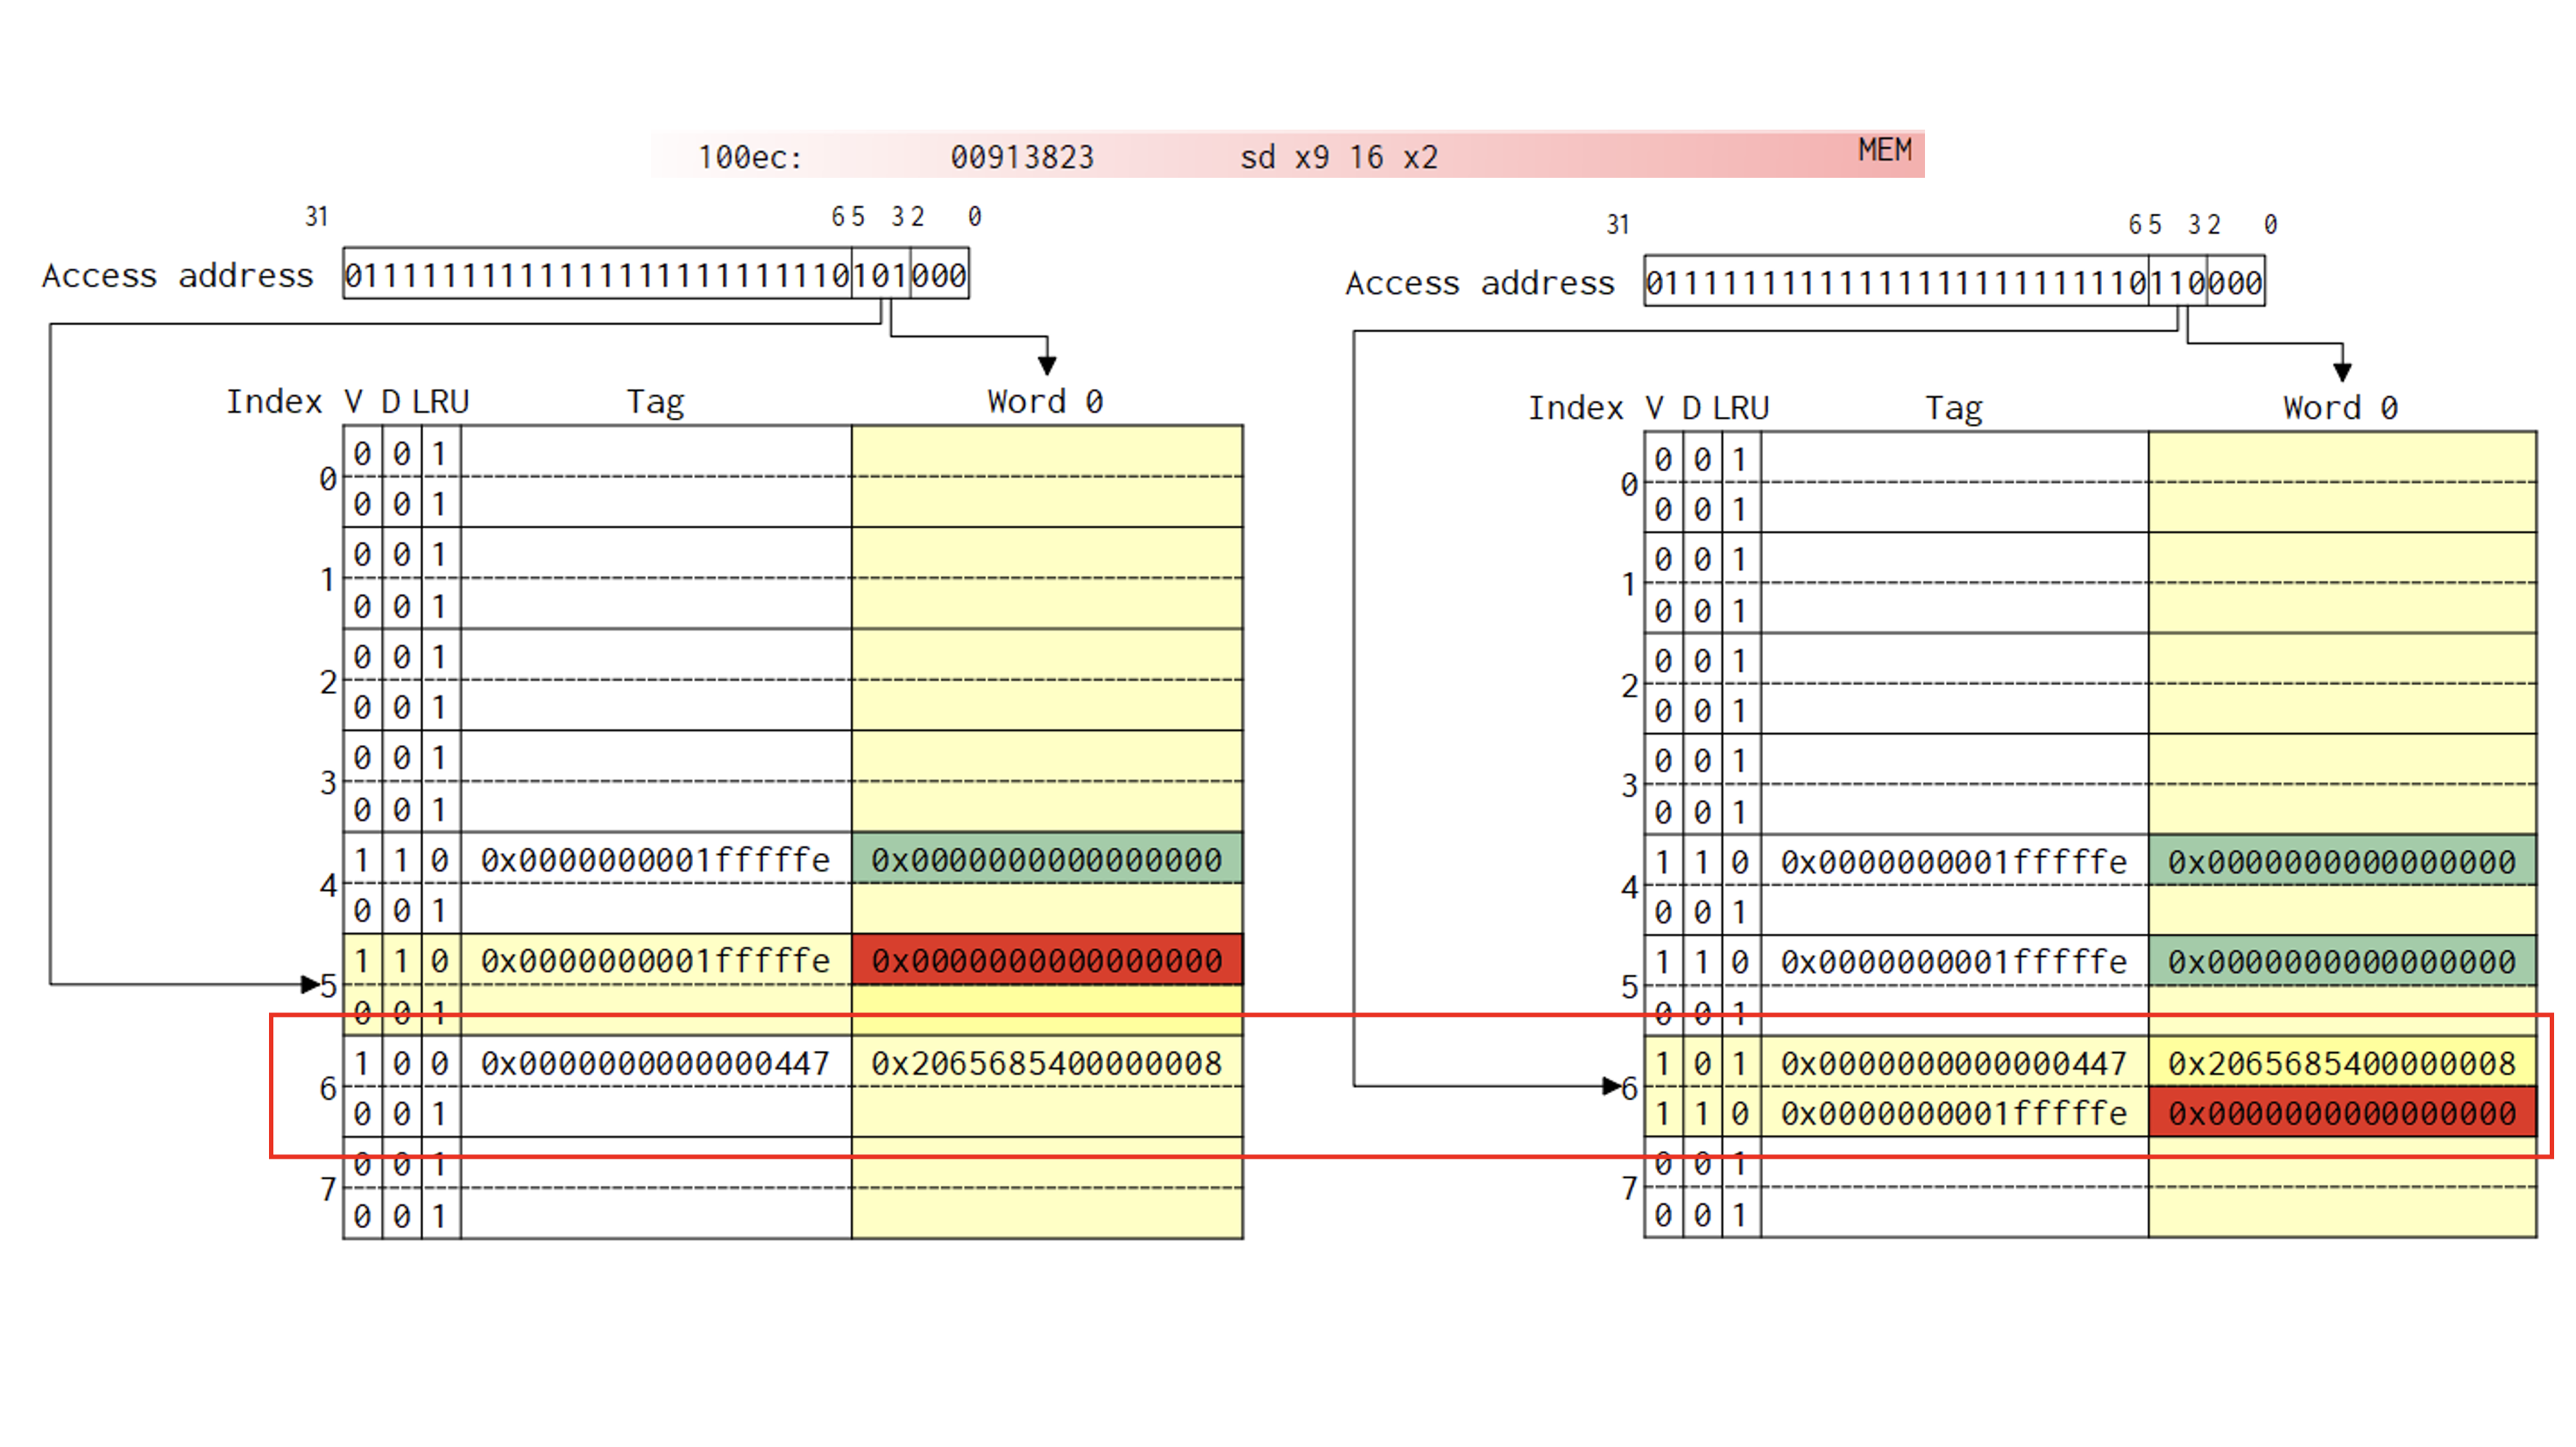
\includegraphics[width=0.8\textwidth]{./img/qa.png}
\end{figure}

This scenario illustrates a \textbf{write miss} at index 6, where one way is already occupied. Due to the write-allocate policy, the block is retrieved from memory and placed in the available way. Following insertion, both the Valid (V) and Dirty (D) bits of this way are set to 1. Regarding the LRU bits, the newly inserted way receives a value of 0 (indicating it's the most recently accessed), while the other way is assigned 1 (signifying it was accessed less recently).

\subsection*{(b)}

\begin{figure}[h!]
    \centering
    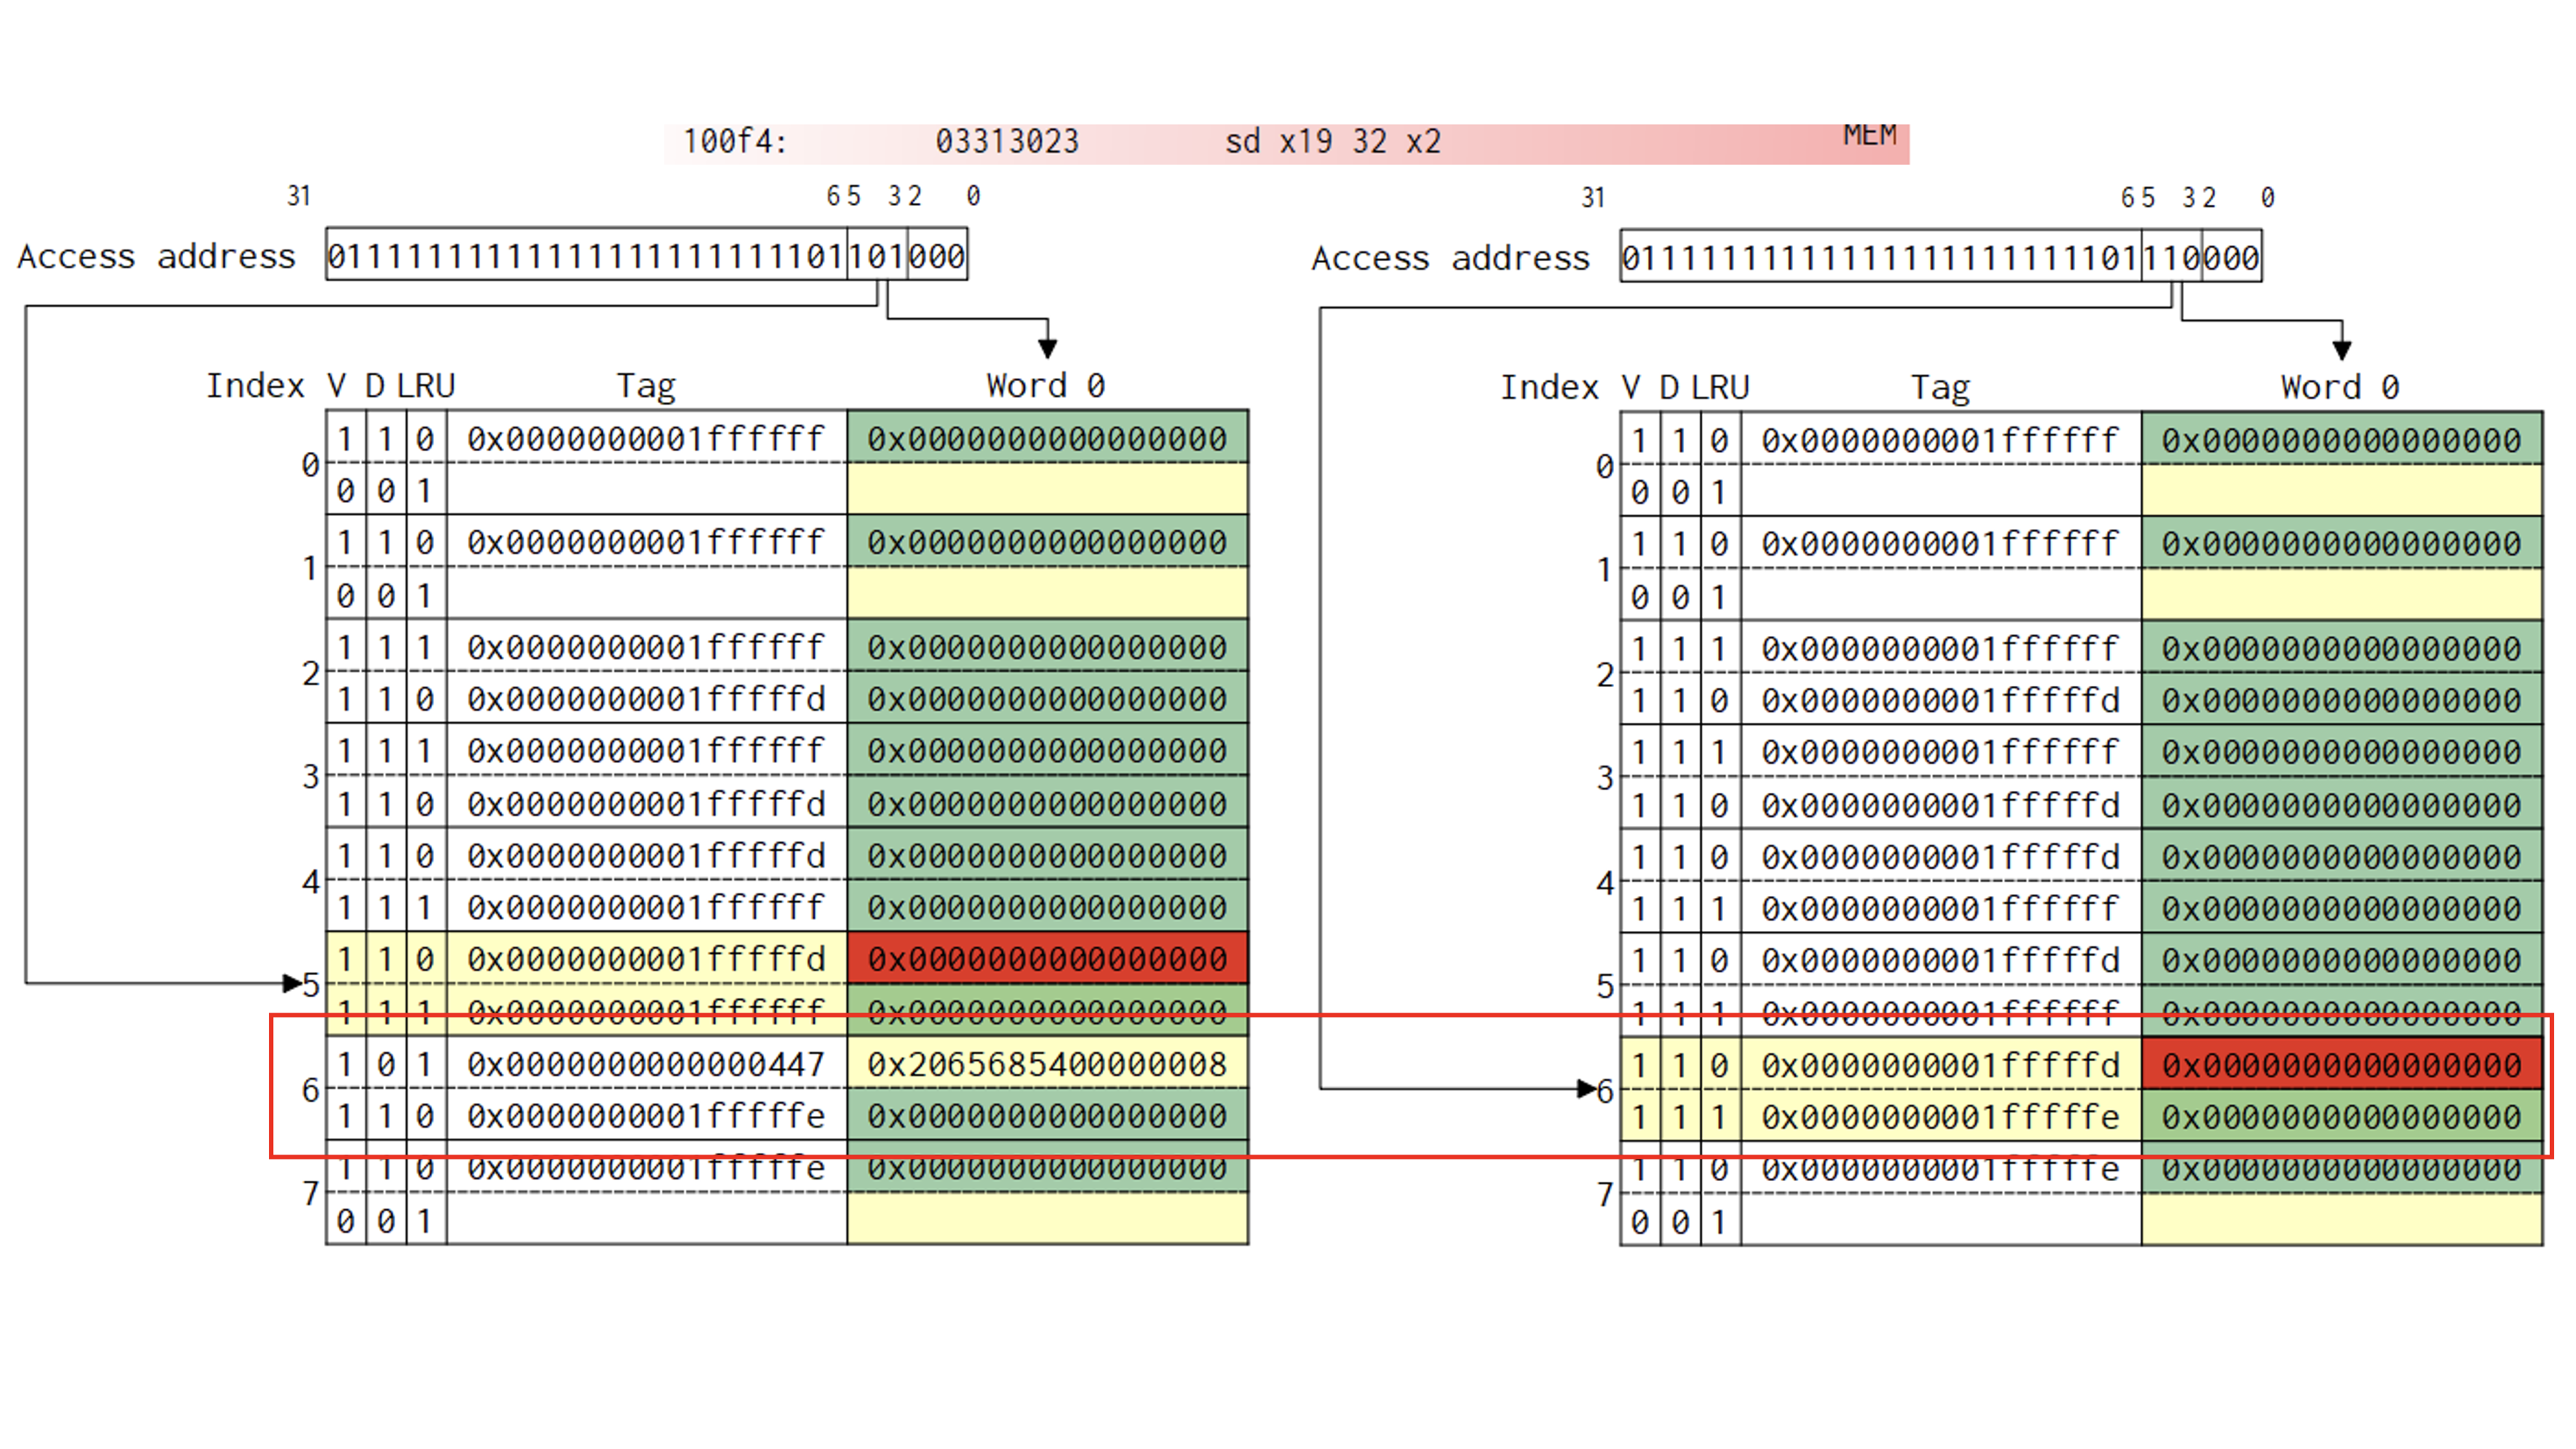
\includegraphics[width=0.8\textwidth]{./img/qb.png}
\end{figure}

This example demonstrates a \textbf{write hit} at index 6, causing the associated block to become dirty. The Dirty bit transitions from 0 to 1, indicating that the block has been modified. Simultaneously, the LRU bit changes from 1 to 0, indicating that this block has just been accessed. When this dirty block eventually needs replacement, a write-back operation will be necessary to preserve the modified data in memory.

\subsection*{(c)}

\begin{figure}[h!]
    \centering
    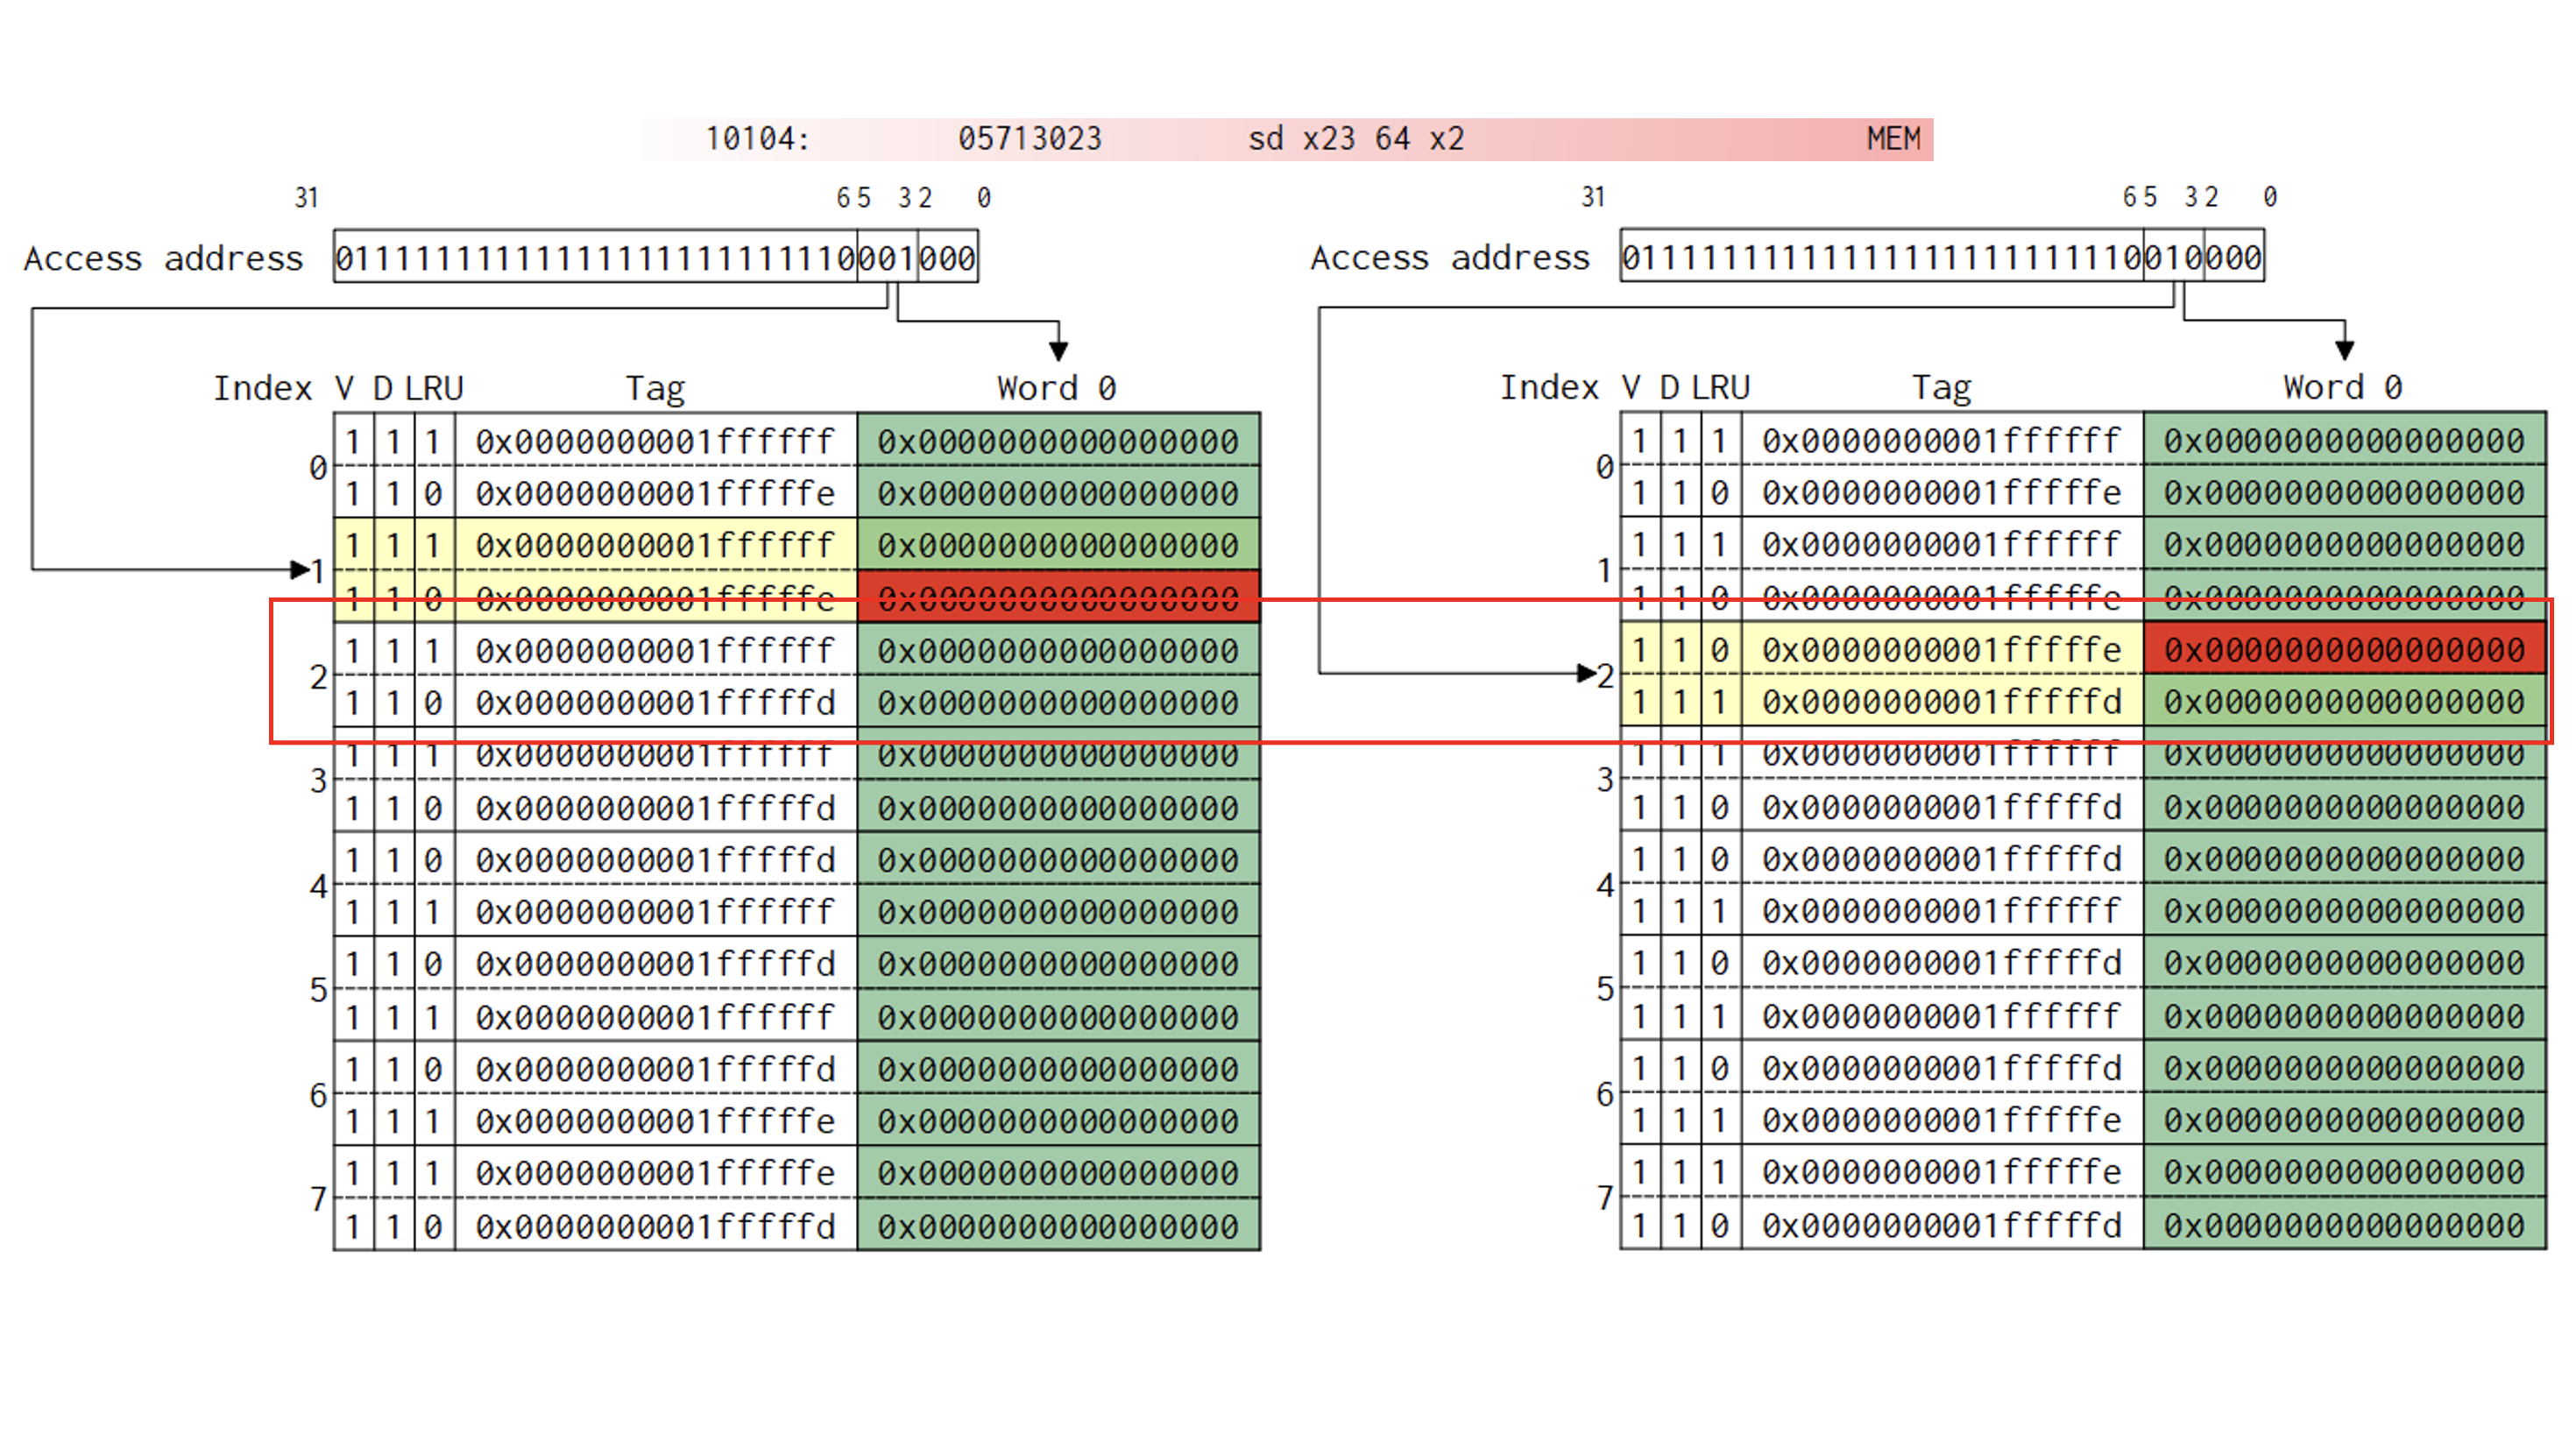
\includegraphics[width=0.8\textwidth]{./img/qc.png}
\end{figure}

In this instance, we observe a \textbf{write miss} at index 2, requiring replacement of a block that must be written back to memory due to its dirty status. Notably, the replaced block had an LRU value of 1, marking it as the least recently used block among the two ways at index 4. This LRU status is precisely what determined this particular block for replacement.

\subsection*{(d)}

After changing the cache configuration to a 4-way set associative design while keeping all other parameters unchanged, the hit rate improved from 0.707 to 0.932. This improvement can be attributed to the increased associativity, which provides more blocks per index. With multiple blocks available at each index, the cache can store more data simultaneously, reducing the frequency of write-backs and misses.

\begin{figure}[h!]
    \centering
    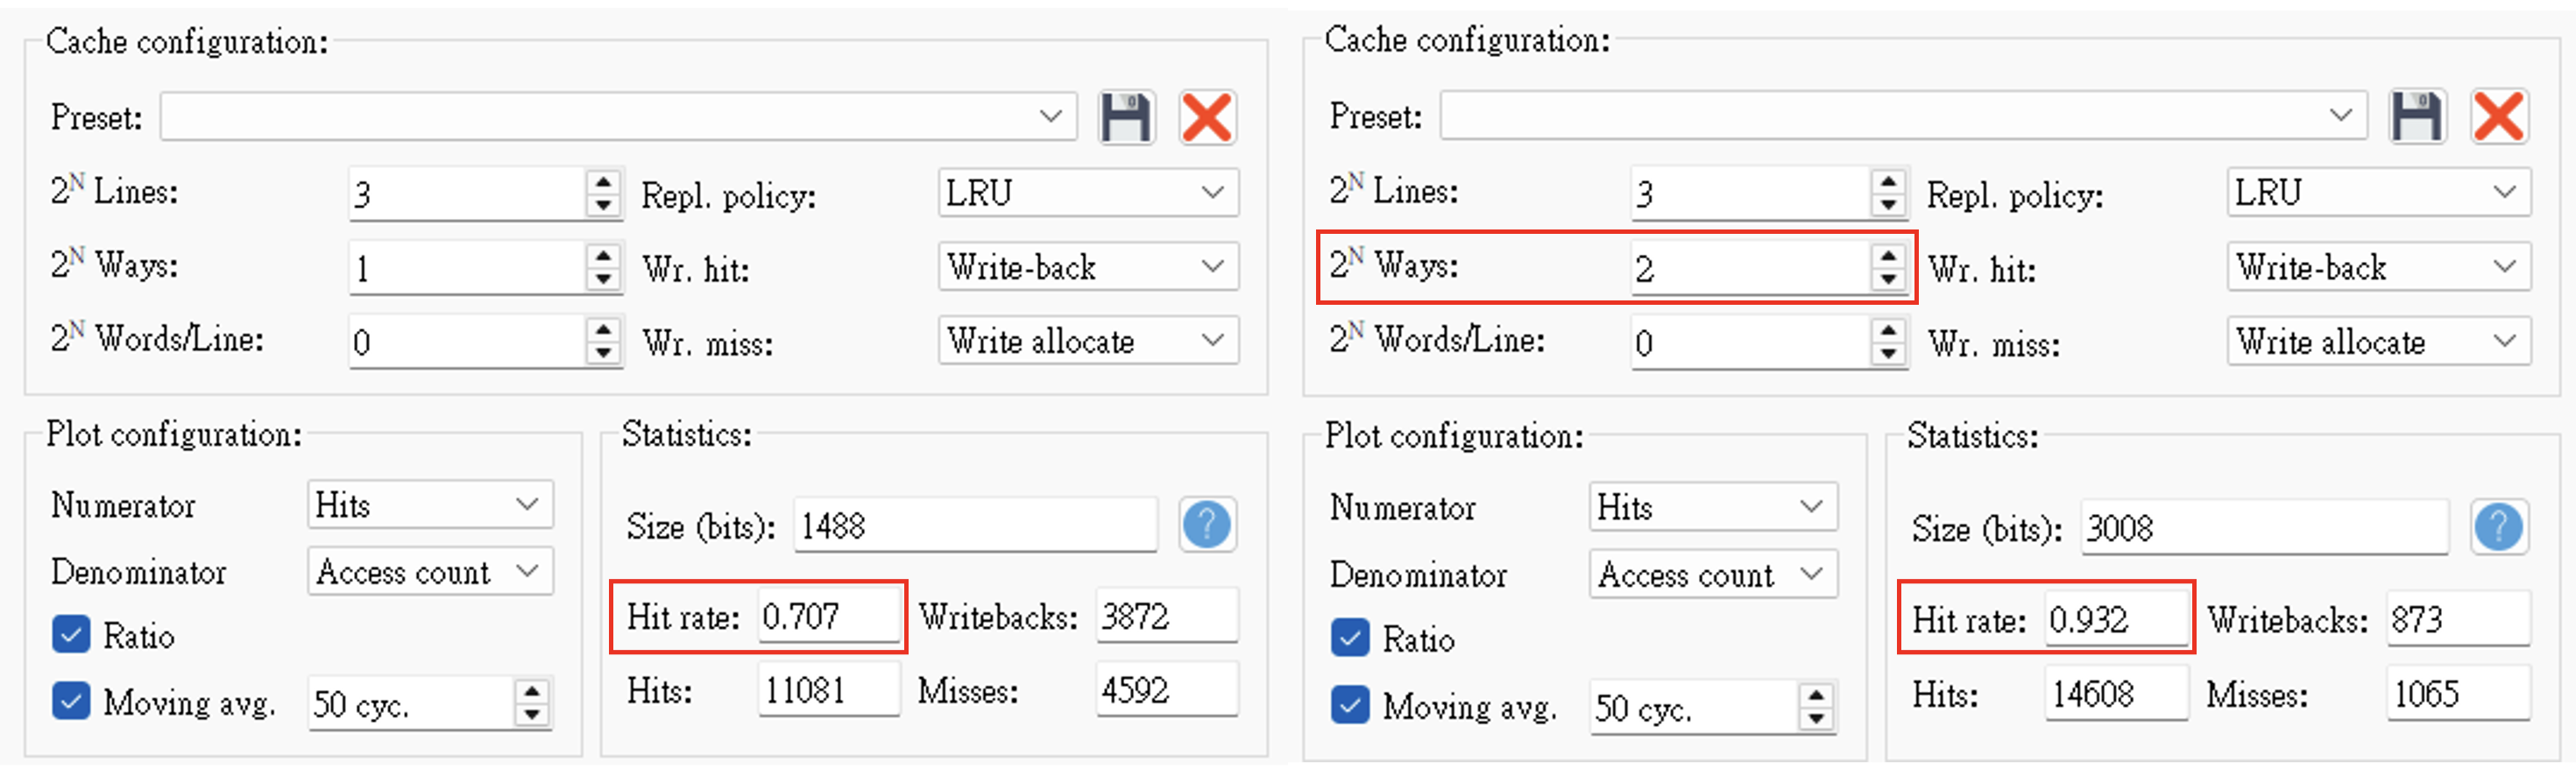
\includegraphics[width=0.8\textwidth]{./img/qd.png}
\end{figure}

\clearpage

\begin{center}
    \large \textbf{Part B: Written Exercises}
\end{center}

\section*{1}

\subsection*{(a)}

\begin{align*}
    \text{Number of block} &= \frac{64 \times 2^{10}}{64} = 1024 \\
    \text{Number of set} &= \frac{1024}{4} = 256
\end{align*}

\subsection*{(b)}

\begin{itemize}
    \item \textbf{Offset:} $6 \text{ bits} \ (\log 64 = 6)$ (2 bits for byte offset, 4 bits for block offset)
    \item \textbf{Index:} $8 \text{ bits} \ (\log 256 = 8)$
    \item \textbf{Tag:} $38 - 6 - 8 = 24 \text{ bits}$
\end{itemize}

\subsection*{(c)}

\begin{align*}
    \text{Total number of KB} &= 1024 \times [1 \text{ (valid)} + 1 \text{ (dirty)} + 24 \text{ (tag)} + 64 \times 8 \text{ (data)}] \\
    &= 550912 \text{ bits} \\
    &= \frac{550912}{8} \text{ bytes} \\
    &= \frac{68864}{1024} \text{ KB} \\
    &= 67.25 \text{ KB}
\end{align*}

\subsection*{(d)}

\begin{align*}
    \text{AMAT} &= \text{Hit time} + \text{Miss rate} \times \text{Miss penalty} \\
    &= 1 + (1 - 0.92) \times 150 \\
    &= 1 + 0.08 \times 150 \\
    &= 1 + 12 \\
    &= 13
\end{align*}

\section*{2}

\subsection*{(a)}

For cache 1 (direct-mapped):

\begin{align*}
    \text{Number of block} &= \frac{256}{8 \times 4} = 8 \\
    \text{Offset bits} &= \log 8 = 3 \\
    \text{Index bits} &= \log 8 = 3 \\
    \text{Tag bits} &= 23 - 3 - 3 = 17 \text{ bits}
\end{align*}

For cache 2 (2-way set associative):

\begin{align*}
    \text{Number of set} &= \frac{256}{(4 \times 4) \times 2} = 8 \\
    \text{Offset bits} &= \log 4 = 2 \\
    \text{Index bits} &= \log 8 = 3 \\
    \text{Tag bits} &= 23 - 3 - 2 = 18 \text{ bits}
\end{align*}

\subsection*{(b)}

For cache 1 (direct-mapped):

\begin{align*}
    \text{bits required} &= [1 \text{ (valid)} + 1 \text{ (dirty)} + 17 \text{ (tag)} + (8 \times 4) \times 8 \text{ (data)}] \times 8 \\
    &= 275 \times 8 = 2200 \text{ bits} \\
\end{align*}

For cache 2 (2-way set associative):

\begin{align*}
    \text{bits required} &= [1 \text{ (valid)} + 1 \text{ (dirty)} + 18 \text{ (tag)} + (4 \times 4) \times 8 \text{ (data)}] \times 16 \\
    &= 148 \times 16 = 2368 \text{ bits}
\end{align*}

\subsection*{(c)}

For cache 1, the references are calculated as follows:

\begin{table}[ht]
    \centering
    \begin{tabular}{|c|c|c|c|c|c|c|}
    \hline
    \textbf{Address} & \textbf{Block} & \textbf{Index} & \textbf{Tag} & \textbf{Hit/Miss} & \textbf{Words in Block} \\ \hline
        60           &  7                     & 7              & 0            & Miss               & 56-63                  \\ \hline
        61           &  7                     & 7              & 0            & Hit                & 56-63                  \\ \hline
        62           &  7                     & 7              & 0            & Hit                & 56-63                  \\ \hline
        68           &  8                     & 0              & 1            & Miss               & 64-71                  \\ \hline
        56           &  7                     & 7              & 0            & Hit                & 56-63                  \\ \hline
        57           &  7                     & 7              & 0            & Hit                & 56-63                  \\ \hline
        32           &  4                     & 4              & 0            & Miss               & 32-39                  \\ \hline
        33           &  4                     & 4              & 0            & Hit                & 32-39                  \\ \hline
        63           &  7                     & 7              & 0            & Hit                & 56-63                  \\ \hline
        64           &  8                     & 0              & 1            & Hit                & 64-71                  \\ \hline
        33           &  4                     & 4              & 0            & Hit                & 32-39                  \\ \hline
        30           &  3                     & 3              & 0            & Miss               & 24-31                  \\ \hline
    \end{tabular}
\end{table}

\clearpage

And the final cache contents for cache 1 are:

\begin{table}[h!]
    \centering
    \begin{tabular}{|c|c|c|}
    \hline
    \textbf{Index} & \textbf{Tag} & \textbf{Words} \\
    \hline
    0              & 1            & 64-71          \\
    \hline
    1              & -            & -              \\
    \hline
    2              & -            & -              \\
    \hline
    3              & 0            & 24-31          \\
    \hline
    4              & 0            & 32-39          \\
    \hline
    5              & -            & -              \\
    \hline
    6              & -            & -              \\
    \hline
    7              & 0            & 56-63          \\
    \hline
    \end{tabular}
\end{table}

For cache 2, the references are calculated as follows:

\begin{table}[ht]
    \centering
        \begin{tabular}{|c|c|c|c|c|c|c|}
        \hline
        \textbf{Address} & \textbf{Block} & \textbf{Index} & \textbf{Tag} & \textbf{Hit/Miss} & \textbf{Placement} & \textbf{Words in Block} \\ \hline
        60               & 15                     & 7              & 1            & Miss              & Way 0              & 60-63                   \\ \hline
        61               & 15                     & 7              & 1            & Hit               & -                  & 60-63                   \\ \hline
        62               & 15                     & 7              & 1            & Hit               & -                  & 60-63                   \\ \hline
        68               & 17                     & 1              & 2            & Miss              & Way 0              & 68-71                   \\ \hline
        56               & 14                     & 6              & 1            & Miss              & Way 0              & 56-59                   \\ \hline
        57               & 14                     & 6              & 1            & Hit               & -                  & 56-59                   \\ \hline
        32               & 8                      & 0              & 1            & Miss              & Way 0              & 32-35                   \\ \hline
        33               & 8                      & 0              & 1            & Hit               & -                  & 32-35                   \\ \hline
        63               & 15                     & 7              & 1            & Hit               & -                  & 60-63                   \\ \hline
        64               & 16                     & 0              & 2            & Miss              & Way 1              & 64-67                   \\ \hline
        33               & 8                      & 0              & 1            & Hit               & -                  & 32-35                   \\ \hline
        30               & 7                      & 7              & 0            & Miss              & Way 1              & 28-31                   \\ \hline
        \end{tabular}
\end{table}

And the final cache contents for cache 2 are:

\begin{table}[h!]
    \centering
    \begin{tabular}{|c|c|c|c|c|}
    \hline
    \multirow{2}{*}{\textbf{Index}} & \multicolumn{2}{c|}{\textbf{Way 0}}     & \multicolumn{2}{c|}{\textbf{Way 1}}     \\
    \cline{2-5}
                                    & \textbf{Tag} & \textbf{Words}          & \textbf{Tag} & \textbf{Words}          \\
    \hline
    0                               & 1            & 32-35                   & 2            & 64-67                   \\
    \hline
    1                               & 2            & 68-71                   & -            & -                       \\
    \hline
    2                               & -            & -                       & -            & -                       \\
    \hline
    3                               & -            & -                       & -            & -                       \\
    \hline
    4                               & -            & -                       & -            & -                       \\
    \hline
    5                               & -            & -                       & -            & -                       \\
    \hline
    6                               & 1            & 56-59                   & -            & -                       \\
    \hline
    7                               & 1            & 60-63                   & 0            & 28-31                   \\
    \hline
    \end{tabular}
\end{table}

\clearpage

\section*{3}

\subsection*{(a)}

The clock rates of P1 and P2 are as follows:

\begin{align*}
    \text{clock\ rate}_\text{P1} = \frac{1}{0.625 \times 10^{-9}} = 1.6 \text{ GHz} \\
    \text{clock\ rate}_\text{P2} = \frac{1}{0.5 \times 10^{-9}} = 2 \text{ GHz}
\end{align*}

\subsection*{(b)}

The AMAT of P1 and P2 are as follows:

\begin{align*}
    \text{AMAT}_\text{P1} &= 0.625 + 0.09 \times 80 = 0.625 + 7.2 = 7.825 \text{ ns} \\
    \text{AMAT}_\text{P2} &= 0.5 + 0.08 \times 80 = 0.5 + 6.4 = 6.9 \text{ ns}
\end{align*}

\subsection*{(c)}

The total CPI of P1 and P2 are as follows:

\begin{align*}
    \text{CPI}_\text{P1} &= 1.0 + 0.09 \times \frac{80}{0.625} \times 0.45 = 6.184 \\
    \text{CPI}_\text{P2} &= 1.0 + 0.08 \times \frac{80}{0.5} \times 0.45 = 6.76 \\
\end{align*}

\subsection*{(d)}

The CPU time of P1 and P2 are as follows:

\begin{align*}
    \text{CPU time}_\text{P1} &= 6.184 \times 0.625 = 3.865 \text{ ns/instruction} \\
    \text{CPU time}_\text{P2} &= 6.76 \times 0.5 = 3.38 \text{ ns/instruction}
\end{align*}

So P2 is faster than P1.

\subsection*{(e)}

After adding L2 cache, the AMAT and CPI of P1 is as follows:

\begin{align*}
    \text{AMAT}_\text{P1} &= 0.625 + 0.09 \times (2.5 + 0.92 \times 80) = 7.474 \text{ ns} \\
    \text{CPI}_\text{P1} &= 1.0 + (0.09 \times \frac{2.5}{0.625} + 0.09 \times 0.92 \times \frac{80}{0.625}) \times 0.45 = 5.93
\end{align*}

Now, comparing the performance of P1 (with L2 cache) and P2 (without L2 cache):

\begin{align*}
    \text{CPU time}_\text{P1} &= 5.93 \times 0.625 = 3.70625 \text{ ns/instruction} \\
    \text{CPU time}_\text{P2} &= 6.76 \times 0.5 = 3.38 \text{ ns/instruction}
\end{align*}

So P2 is faster than P1.

\subsection*{(f)}

Denote the required L1 miss rate for P1 as $x$.

The CPI for P1 would be:
\begin{align*}
    \text{CPI}_\text{P1} &= 1.0 + x \times \frac{80}{0.625} \times 0.45 \\
    &= 1.0 + x \times 128 \times 0.45 \\
    &= 1.0 + 57.6x
\end{align*}

For P1 to match P2's performance, their CPU times must be equal:
\begin{align*}
    \text{CPU time}_\text{P1} &= \text{CPU time}_\text{P2} \\
    \text{CPI}_\text{P1} \times 0.625 &= 3.38 \\
    \text{CPI}_\text{P1} &= \frac{3.38}{0.625} = 5.408
\end{align*}

Substituting this CPI value:
\begin{align*}
    5.408 &= 1.0 + 57.6x \\
    4.408 &= 57.6x \\
    x &= \frac{4.408}{57.6} \approx 0.0765
\end{align*}

Therefore, P1 would require an L1 miss rate of approximately 0.0765 (7.65\%) to match P2's performance.

\section*{4}

\subsection*{(a)}

For L1 data TLB:
\begin{itemize}
    \item \textbf{Page Offset:} $13 \text{ bits} \ (\text{page size} = 8 \text{ KB} = 2^{13} \text{ bytes})$
    \item \textbf{Virtual Page Number (VPN):} $42 - 13 = 29 \text{ bits}$
\end{itemize}

Since L1 TLB is fully associative with 128 entries, the entire VPN serves as the tag.

\begin{table}[h]
    \centering
    \begin{tabular}{|c|c|c|}
    \hline
    \textbf{Field} & \textbf{Bits} & \textbf{Size} \\
    \hline
    Virtual Page Number (VPN) & [41:13] & 29 bits \\
    \hline
    Page Offset & [12:0] & 13 bits \\
    \hline
    \end{tabular}
\end{table}

\subsection*{(b)}

For L2 TLB (4-way set associative with 512 entries = 128 sets):
\begin{itemize}
    \item \textbf{Page Offset:} $13 \text{ bits}$
    \item \textbf{Index:} $\log 128 = 7 \text{ bits}$
    \item \textbf{Tag:} $42 - 13 - 7 = 22 \text{ bits}$
\end{itemize}

\begin{table}[h]
    \centering
    \begin{tabular}{|c|c|c|}
    \hline
    \textbf{Field} & \textbf{Bits} & \textbf{Size} \\
    \hline
    Tag & [41:20] & 22 bits \\
    \hline
    Index & [19:13] & 7 bits \\
    \hline
    Page Offset & [12:0] & 13 bits \\
    \hline
    \end{tabular}
\end{table}

\subsection*{(c)}

For L1 data cache (32 KB, 2-way set associative, 128-byte blocks):
\begin{itemize}
    \item \textbf{Block Offset:} $\log 128 = 7 \text{ bits}$
    \item \textbf{Index:} $\log \frac{32 \times 2^{10}}{128 \times 2} = \log 128 = 7 \text{ bits}$
    \item \textbf{Tag:} $36 - 7 - 7 = 22 \text{ bits}$
\end{itemize}

\begin{table}[h]
    \centering
    \begin{tabular}{|c|c|c|}
    \hline
    \textbf{Field} & \textbf{Bits} & \textbf{Size} \\
    \hline
    Tag & [35:14] & 22 bits \\
    \hline
    Index & [13:7] & 7 bits \\
    \hline
    Block Offset & [6:0] & 7 bits \\
    \hline
    \end{tabular}
\end{table}

\subsection*{(d)}

For L2 cache (512 KB, 4-way set associative, 128-byte blocks):
\begin{itemize}
    \item \textbf{Block Offset:} $\log 128 = 7 \text{ bits}$
    \item \textbf{Index:} $\log \frac{512 \times 2^{10}}{128 \times 4} = \log 1024 = 10 \text{ bits}$
    \item \textbf{Tag:} $36 - 7 - 10 = 19 \text{ bits}$
\end{itemize}

\begin{table}[h]
    \centering
    \begin{tabular}{|c|c|c|}
    \hline
    \textbf{Field} & \textbf{Bits} & \textbf{Size} \\
    \hline
    Tag & [35:17] & 19 bits \\
    \hline
    Index & [16:7] & 10 bits \\
    \hline
    Block Offset & [6:0] & 7 bits \\
    \hline
    \end{tabular}
\end{table}

\section*{5}

\subsection*{(a)}

\begin{table}[htbp]
    \centering
    \begin{tabular}{|c|c|c|c|c|c|c|}
    \hline
    p1 & p2 & d1 & p4 & d2 & d3 & d4 \\
    \hline
       &    & 1  &    & 0  & 1  & 0  \\
    \hline
    1  &    & 1  &    & 0  & 1  & 0  \\
    \hline
    1  & 0  & 1  &    & 0  & 1  & 0  \\
    \hline
    1  & 0  & 1  & 1  & 0 & 1 & 0 \\
    \hline
    \end{tabular}
\end{table}

\begin{align*}
    p_1 &= d_1 \oplus d_2 \oplus d_4 = 1 \oplus 0 \oplus 0 = 1 \\
    p_2 &= d_1 \oplus d_3 \oplus d_4 = 1 \oplus 1 \oplus 0 = 0 \\
    p_4 &= d_2 \oplus d_3 \oplus d_4 = 0 \oplus 1 \oplus 0 = 1
\end{align*}

So the codeword is 1011010.

\subsection*{(b)}

For SECDED (Single Error Correcting, Double Error Detecting), we add an additional overall parity bit $p_n$ to the Hamming code.

\begin{table}[htbp]
    \centering
    \begin{tabular}{|c|c|c|c|c|c|c|c|}
    \hline
    p1 & p2 & d1 & p4 & d2 & d3 & d4 & pn \\
    \hline
       &    & 1  &    & 1  & 0  & 1  &    \\
    \hline
    1  &    & 1  &    & 1  & 0  & 1  &    \\
    \hline
    1  & 0  & 1  &    & 1  & 0  & 1  &    \\
    \hline
    1  & 0  & 1  & 0  & 1  & 0  & 1  &    \\
    \hline
    1  & 0  & 1  & 0  & 1  & 0  & 1  & 0  \\
    \hline
    \end{tabular}
\end{table}

\begin{align*}
    p_1 &= d_1 \oplus d_2 \oplus d_4 = 1 \oplus 1 \oplus 1 = 1 \\
    p_2 &= d_1 \oplus d_3 \oplus d_4 = 1 \oplus 0 \oplus 1 = 0 \\
    p_4 &= d_2 \oplus d_3 \oplus d_4 = 1 \oplus 0 \oplus 1 = 0 \\
    p_n &= p_1 \oplus p_2 \oplus d_1 \oplus p_4 \oplus d_2 \oplus d_3 \oplus d_4 = 1 \oplus 0 \oplus 1 \oplus 0 \oplus 1 \oplus 0 \oplus 1 = 0
\end{align*}

So the SECDED codeword is 10101010.

\subsection*{(c)}

\begin{align*}
    h_1 &= 0 \oplus 1 \oplus 0 \oplus 0 = 1 \\
    h_2 &= 1 \oplus 1 \oplus 1 \oplus 0 = 1 \\
    h_4 &= 0 \oplus 0 \oplus 1 \oplus 0 = 1 \\
    H &= h_4h_2h_1 = 111_{2} = 7 \\
    h_n &= 0 \oplus 1 \oplus 1 \oplus 0 \oplus 0 \oplus 1 \oplus 0 \oplus 0 = 1 \text{ (parity of whole word)}
\end{align*}

Since $H \neq 0$ and $h_n$ is odd, there is a single error at position 7. Therefore, the corrected codeword is 01100110.

\subsection*{(d)}

\begin{align*}
    h_1 &= 1 \oplus 1 \oplus 0 \oplus 0 = 0 \\
    h_2 &= 1 \oplus 1 \oplus 1 \oplus 0 = 1 \\
    h_4 &= 1 \oplus 0 \oplus 1 \oplus 0 = 0 \\
    H &= h_4h_2h_1 = 010_{2} = 2 \\
    h_n &= 1 \oplus 1 \oplus 1 \oplus 1 \oplus 0 \oplus 1 \oplus 0 \oplus 1 = 0 \text{ (parity of whole word)}
\end{align*}

Since $H \neq 0$ and $h_n$ is even, this codeword contains two errors that can be detected but not corrected.

\subsection*{(e)}

To protect 96 bits of data using SECDED, we need:

\begin{align*}
    2^p \geq 96 + p + 1
\end{align*}

Testing values of $p$ for the Hamming code part:

\begin{itemize}
    \item For $p = 6$: $2^6 = 64 < 96 + 6 + 1 = 103$
    \item For $p = 7$: $2^7 = 128 \geq 96 + 7 + 1 = 104$
\end{itemize}

So we need 7 parity bits for single error correction. Since SECDED requires an additional overall parity bit, the minimum number of parity bits required is $7 + 1 = 8$.

\end{document}